\section{Конструкторский раздел}

В данном разделе представлена архитектура программного обеспечения. Приведен концептуальный и логический дизайн системы, а также сценарии функционирования системы.

\subsection{Концептуальный дизайн}

На рисунке \ref{img:idef} представлена IDEF-0 диаграмма, обеспечивающая наиболее абстрактное описание работы системы.

\begin{figure}[H]
	\centering
	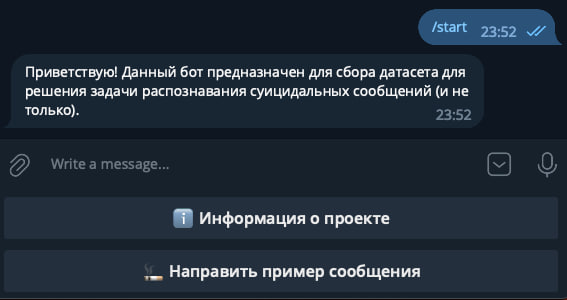
\includegraphics[width=\textwidth]{inc/1.pdf}
	\caption{ Диаграмма IDEF-0, описывающая работу системы.}
	\label{img:idef}
\end{figure}


На рисунке \ref{img:idef1} представлена IDEF-0 диаграмма, уточняющая детали работы системы при обработке запроса на анализ сообщения.

\begin{figure}[H]
	\centering
	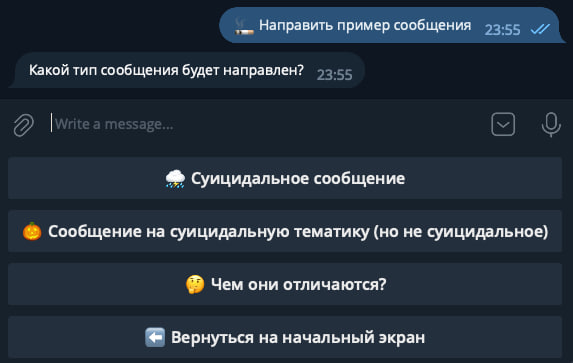
\includegraphics[width=\textwidth]{inc/2.pdf}
	\caption{ Диаграмма IDEF-0, описывающая работу системы.}
	\label{img:idef1}
\end{figure}

\subsection{Сценарии функционирования системы}
Далее приведены подробные сценарии основных возможных действий пользователя.

\textbf{Регистрация пользователя:}
\begin{enumerate}
\item Пользователь нажимает на кнопку ``Зарегистрироваться'' в интерфейсе приложения;
\item Пользователю открывается форма, которая содержит поля для заполнения ФИО, адреса электронной почты и пароля;
\item Пользователь вводит данные в форму и для завершения регистрации нажимает на кнопку ``Зарегистрироваться'', тем самым подтверждая верность своих данных и согласие на их обработку и хранение;
\item Если пользователь с введенным для регистрации логином уже существует, то высвечивается ошибка; При успешной регистрации пользователь перенаправляется на экран входа в приложение.
\end{enumerate}


\textbf{Авторизация пользователя:}
\begin{enumerate}
\item Пользователю открывается форма, которая содержит поля для заполнения логина и пароля;
\item Пользователь завершает работу с формой авторизации нажатием кнопки ``Войти'' в интерфейсе приложения;
\item При обнаружении ошибки в данных, пользователю высвечивается сообщении, о том, что пользователь не найден; при совпадении данных с записью в базе данных аккаунтов пользователь получает доступ к системе.
\end{enumerate}

\textbf{Анализ сообщения:}
\begin{enumerate}
\item Авторизованный пользователь на главном экране приложения нажимает на кнопку ``Проверить сообщение'';
\item Пользователь перенаправляется на форму, которая содержит поля ``Сообщение'' и ``Имя наблюдаемого'';
\item После заполнения формы пользователь и нажатия на кнопку ``Проверить'' пользователь перенаправляется на экран, содержащий в себе информацию о том, является ли сообщение несуицидальным; В случае, если сообщение можно отнести к суицидальному, на экране также выводится рекомендация.
\end{enumerate}

\subsection{Диаграммы прецедентов}

На рисунке \ref{img:usecase} представлена диаграмма вариантов использования системы для ролей пользователь и администратор.

\begin{figure}[H]
	\centering
	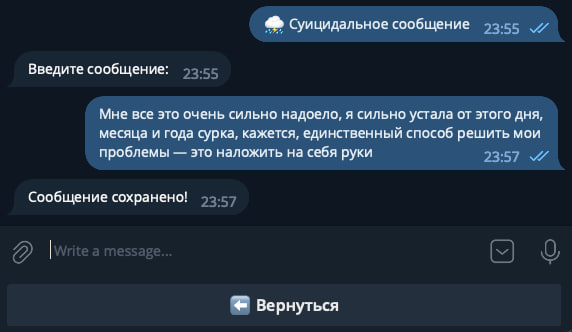
\includegraphics[width=\textwidth]{inc/3.pdf}
	\caption{ Диаграмма вариантов использования системы.}
	\label{img:usecase}
\end{figure}

\subsection{Спецификации сценариев}

\textbf{Спецификация сценария ``Регистрация''}

\begin{table}[H]
\begin{center}
\begin{tabular}{|C{8cm}C{8cm}|}
\hline
\multicolumn{2}{|C{16cm}|}{\textbf{Нормальный ход сценария}}    \\ \hline
\multicolumn{1}{|C{8cm}|}{\textbf{Действие пользователя}} & \textbf{Отклик системы} \\ \hline
\multicolumn{1}{|C{8cm}|}{Пользователь нажимает кнопку ``Зарегистрироваться''} & Открывается форма для заполнения данных \\ \hline
\multicolumn{1}{|C{8cm}|}{Пользователь вводит данные в поля и нажимает кнопку ``Зарегистрироваться''} & Пользователь перенаправляется на экран входа в приложение  \\ \hline
\end{tabular}
\end{center}
\end{table}

\begin{table}[H]
\begin{center}
\begin{tabular}{|C{8cm}C{8cm}|}
\hline
\multicolumn{2}{|C{16cm}|}{\textbf{Альтернативный ход сценария}}    \\ \hline
\multicolumn{1}{|C{8cm}|}{\textbf{Действие пользователя}} & \textbf{Отклик системы} \\ \hline
\multicolumn{1}{|C{8cm}|}{Пользователь нажимает кнопку ``Зарегистрироваться''} &  Открывается форма для заполнения данных \\ \hline
\multicolumn{1}{|C{8cm}|}{Пользователь вводит данные в поля и нажимает кнопку ``Зарегистрироваться''} & На экране появляется сообщение ``Такой пользователь уже существует'' \\ \hline
\end{tabular}
\end{center}
\end{table}

\textbf{Спецификация сценария ``Авторизация''}

\begin{table}[H]
\begin{center}
\begin{tabular}{|C{8cm}C{8cm}|}
\hline
\multicolumn{2}{|C{16cm}|}{\textbf{Нормальный ход сценария}}    \\ \hline
\multicolumn{1}{|C{8cm}|}{\textbf{Действие пользователя}} & \textbf{Отклик системы} \\ \hline
\multicolumn{1}{|C{8cm}|}{Пользователь нажимает кнопку ``Войти''} & Открывается форма для ввода данных \\ \hline
\multicolumn{1}{|C{8cm}|}{Пользователь заполняет форму и нажимает кнопку ``Войти''} & Открывается главная страница приложения \\ \hline
\end{tabular}
\end{center}
\end{table}

\begin{table}[H]
\begin{center}
\begin{tabular}{|C{8cm}C{8cm}|}
\hline
\multicolumn{2}{|C{16cm}|}{\textbf{Альтернативный ход сценария}}    \\ \hline
\multicolumn{1}{|C{8cm}|}{\textbf{Действие пользователя}} & \textbf{Отклик системы} \\ \hline
\multicolumn{1}{|C{8cm}|}{Пользователь нажимает кнопку ``Войти''} & Открывается форма для ввода данных \\ \hline
\multicolumn{1}{|C{8cm}|}{Пользователь заполняет форму и нажимает кнопку ``Войти''} & На экране появляется сообщение ``Неверный логин или пароль'' \\ \hline
\end{tabular}
\end{center}
\end{table}

\textbf{Спецификация сценария ``Анализ сообщения''}

\begin{table}[H]
\begin{center}
\begin{tabular}{|C{8cm}C{8cm}|}
\hline
\multicolumn{2}{|C{16cm}|}{\textbf{Нормальный ход сценария}}    \\ \hline
\multicolumn{1}{|C{8cm}|}{\textbf{Действие пользователя}} & \textbf{Отклик системы} \\ \hline
\multicolumn{1}{|C{8cm}|}{Пользователь заполняет форму и нажимает кнопку ``Проанализировать'' } & Пользователь перенаправляется на экран с результатами анализа \\ \hline
\end{tabular}
\end{center}
\end{table}

\begin{table}[H]
\begin{center}
\begin{tabular}{|C{8cm}C{8cm}|}
\hline
\multicolumn{2}{|C{16cm}|}{\textbf{Альтернативный ход сценария}}    \\ \hline
\multicolumn{1}{|C{8cm}|}{\textbf{Действие пользователя}} & \textbf{Отклик системы} \\ \hline
\multicolumn{1}{|C{8cm}|}{Пользователь заполняет форму и нажимает кнопку ``Проанализировать'' } & На экране появляется сообщение ``Сообщение не может быть пустым'' \\ \hline
\end{tabular}
\end{center}
\end{table}

\subsection{Логический дизайн}
На рисунке \ref{img:er} представлена ER-диаграмма в нотации Чена, построенная на основе функциональных требований к выделенным подсистемам, а также объектов, о которых необходимо хранить данные в системе информацию.

\begin{figure}[H]
	\centering
	
\includegraphics[width=\textwidth]{inc/4.pdf}
	\caption{ ER-диаграмма.}
	\label{img:er}
\end{figure}

На рисунке \ref{img:bd} представлена схема базы данных системы.

\begin{figure}[H]
	\centering
	\includegraphics[width=\textwidth]{inc/5.pdf}
	\caption{ Схема базы данных системы.}
	\label{img:bd}
\end{figure}

Далее приведены спецификации тиблиц базы данных, приведенных на рисунке \ref{img:bd}.

\textbf{Спецификация таблицы Пользователь}

\begin{table}[H]
\begin{center}
\begin{tabular}{|C{4cm}|C{4cm}|C{6cm}|}
\hline
\textbf{Имя атрибута} & \textbf{Тип атрибута} & \textbf{Описание атрибута} \\ \hline
id & UUID & Идентификатор пользователя \\ \hline
name & String & ФИО пользователя \\ \hline
mail & String & электронная почта пользователя \\ \hline
password & String & Пароль пользователя \\ \hline
role & String & Роль (клиент или администратор) \\ \hline
\end{tabular}
\end{center}
\end{table}

\pagebreak

\textbf{Спецификация таблицы Наблюдаемый пользователь}

\begin{table}[H]
\begin{center}
\begin{tabular}{|C{4cm}|C{4cm}|C{6cm}|}
\hline
\textbf{Имя атрибута} & \textbf{Тип атрибута} & \textbf{Описание атрибута} \\ \hline
id & UUID & Идентификатор наблюдаемого пользователя \\ \hline
masterId & UUID & Идентификатор направителя сообщений пользователя \\ \hline
name & String & Псевдоним пользователя \\ \hline
\end{tabular}
\end{center}
\end{table}

\textbf{Спецификация таблицы Сообщение}

\begin{table}[H]
\begin{center}
\begin{tabular}{|C{4cm}|C{4cm}|C{6cm}|}
\hline
\textbf{Имя атрибута} & \textbf{Тип атрибута} & \textbf{Описание атрибута} \\ \hline
id & UUID & Идентификатор сообщения \\ \hline
masterId & UUID & Идентификатор пользователя, направившего сообщение в систему \\ \hline
watchUserId & UUID & Идентификатор наблюдаемого пользователя \\ \hline
message & String & Сообщение пользователя \\ \hline
\end{tabular}
\end{center}
\end{table}

\textbf{Спецификация таблицы Рекомендация}
\begin{table}[H]
\begin{center}
\begin{tabular}{|C{4cm}|C{4cm}|C{6cm}|}
\hline
\textbf{Имя атрибута} & \textbf{Тип атрибута} & \textbf{Описание атрибута} \\ \hline
id & UUID & Идентификатор рекомендации \\ \hline
text & String & Текст рекомендации \\ \hline
state & String & Состояние пользователя, соотнесенное рекомендации \\ \hline
\end{tabular}
\end{center}
\end{table}

\subsection{Структура сервиса анализа и сбора данных}

На рисунке \ref{img:anal} представлена диаграмма классов для разработки сервиса агрегации запросов.

\begin{figure}[H]
	\centering
	\includegraphics[width=\textwidth]{inc/6.pdf}
	\caption{ Структура сервиса агрегации запросов.}
	\label{img:anal}
\end{figure}

Функциональные требования, предъявляемые к сервису агрегации запросов, реализуются с использованием методов контроллера AgregationController.

\textbf{Спецификация класса AgregationController}

\begin{table}[H]
\begin{center}
\begin{tabular}{|C{8cm}|C{8cm}|}
\hline
\textbf{Метод} & \textbf{Назначение} \\ \hline
check & Проверка работоспособности сервиса \\ \hline
register & Регистрация пользователя \\ \hline
auth & Авторизация \\ \hline
analyzeMessage & Анализ сообщения на наличие суицидальных маркеров \\ \hline
saveMessage & Сохранение сообщения в БД несуицидальных сообщений \\ \hline
addWatchUserMessage & Добавление сообщений наблюдаемого пользователя \\ \hline
getRecommendation & Получение рекомендации по указанному состоянию \\ \hline
deleteUser & Удаление пользователя \\ \hline
\end{tabular}
\end{center}
\end{table}

\subsection{Диаграмма последовательности действий}

На рисунке \ref{img:timeline} изображен процесс получения результатов анализа сообщения пользователем с указанием наблюдаемого пользователя.

\begin{figure}[H]
	\centering
	\includegraphics[width=\textwidth]{inc/7.pdf}
	\caption{ Диаграмма последовательности действий при запросе пользователя анализа сообщения с указанием наблюдаемого пользователя.}
	\label{img:timeline}
\end{figure}

\subsection{Диаграмма потоков данных}

На рисунке \ref{img:flows} представлена диаграмма потоков данных при запросе пользователем результатов анализа сообщения.

\begin{figure}[H]
	\centering
	\includegraphics[width=\textwidth]{inc/8.pdf}
	\caption{ Диаграмма потоков данных при запросе пользователем результатов анализа сообщения.}
	\label{img:flows}
\end{figure}

\pagebreak